\documentclass[11pt]{article}

\usepackage[a4paper,margin=1in]{geometry}
\usepackage{graphicx}
\usepackage{hyperref}
\usepackage[T1]{fontenc}
\usepackage{lmodern}
\usepackage{enumitem}
\usepackage{xcolor}
\usepackage{listings}

\hypersetup{
  colorlinks=true,
  linkcolor=blue,
  urlcolor=blue
}

\lstset{
  basicstyle=\ttfamily\small,
  breaklines=true,
  frame=single,
  backgroundcolor=\color{black!3}
}

\title{Coding Challenge - Broadening the RISC-V High Precision Code Base and Reach}
\author{}
\date{\today}

\begin{document}

\maketitle

\section{Overview}

This submission provides two small Bash-based demonstrations for the assignment prompt:

\begin{itemize}[leftmargin=1.5em]
  \item \texttt{hanoi.sh}: a Tower of Hanoi implementation
  \item \texttt{life.sh}: a Conway's Game of Life implementation
\end{itemize}

Both scripts were written in a scripted language, include simple graphics in the terminal, and clearly mark the sections that demonstrate recursion and iteration.

\section{Repository and Website Links}

The full submission is available in two forms:

\begin{itemize}[leftmargin=1.5em]
  \item Repository: \url{https://github.com/Sanchay117/terminal-game-of-life}
  \item Live website: \url{https://sanchay117.github.io/terminal-game-of-life/}
\end{itemize}

The repository contains the original Bash challenge deliverables, screenshots, deployment workflow, and the browser-facing website code. The live website provides a public demonstration layer that is easier to share and review.

\section{Assignment Prompt}

The assignment requested the following:

\begin{quote}
Please create a ``Tower Of Hanoi'' or ``Conway's Game of Life'' code demonstration in a scripted language or bash script. This can be short, just enough to demonstrate functionality with simple graphics. Ideally, you can identify and comment on the sections that demonstrate recursion and / or iteration. Optionally, place it on a publicly accessible github site.
\end{quote}

This repository satisfies the request by implementing \emph{both} challenge options in Bash, and by additionally including an optional GitHub Pages site for public presentation.

\section{Tower of Hanoi Demo}

The Tower of Hanoi implementation is contained in \texttt{hanoi.sh}. It displays the peg contents after each move using simple ASCII graphics. Disks are rendered with \texttt{=} characters and the state is updated step by step.

\subsection{Concept Demonstrated}

The key algorithmic concept demonstrated here is \textbf{recursion}. The function \texttt{solve\_hanoi()} breaks the problem into smaller subproblems:

\begin{enumerate}[leftmargin=1.5em]
  \item move the top \(n-1\) disks to the auxiliary peg,
  \item move the largest disk to the destination peg,
  \item move the \(n-1\) disks from the auxiliary peg to the destination peg.
\end{enumerate}

This recursive structure is also labeled directly in the code comments to make the technique easy to identify.

\subsection{Example Output}

\begin{figure}[h]
  \centering
  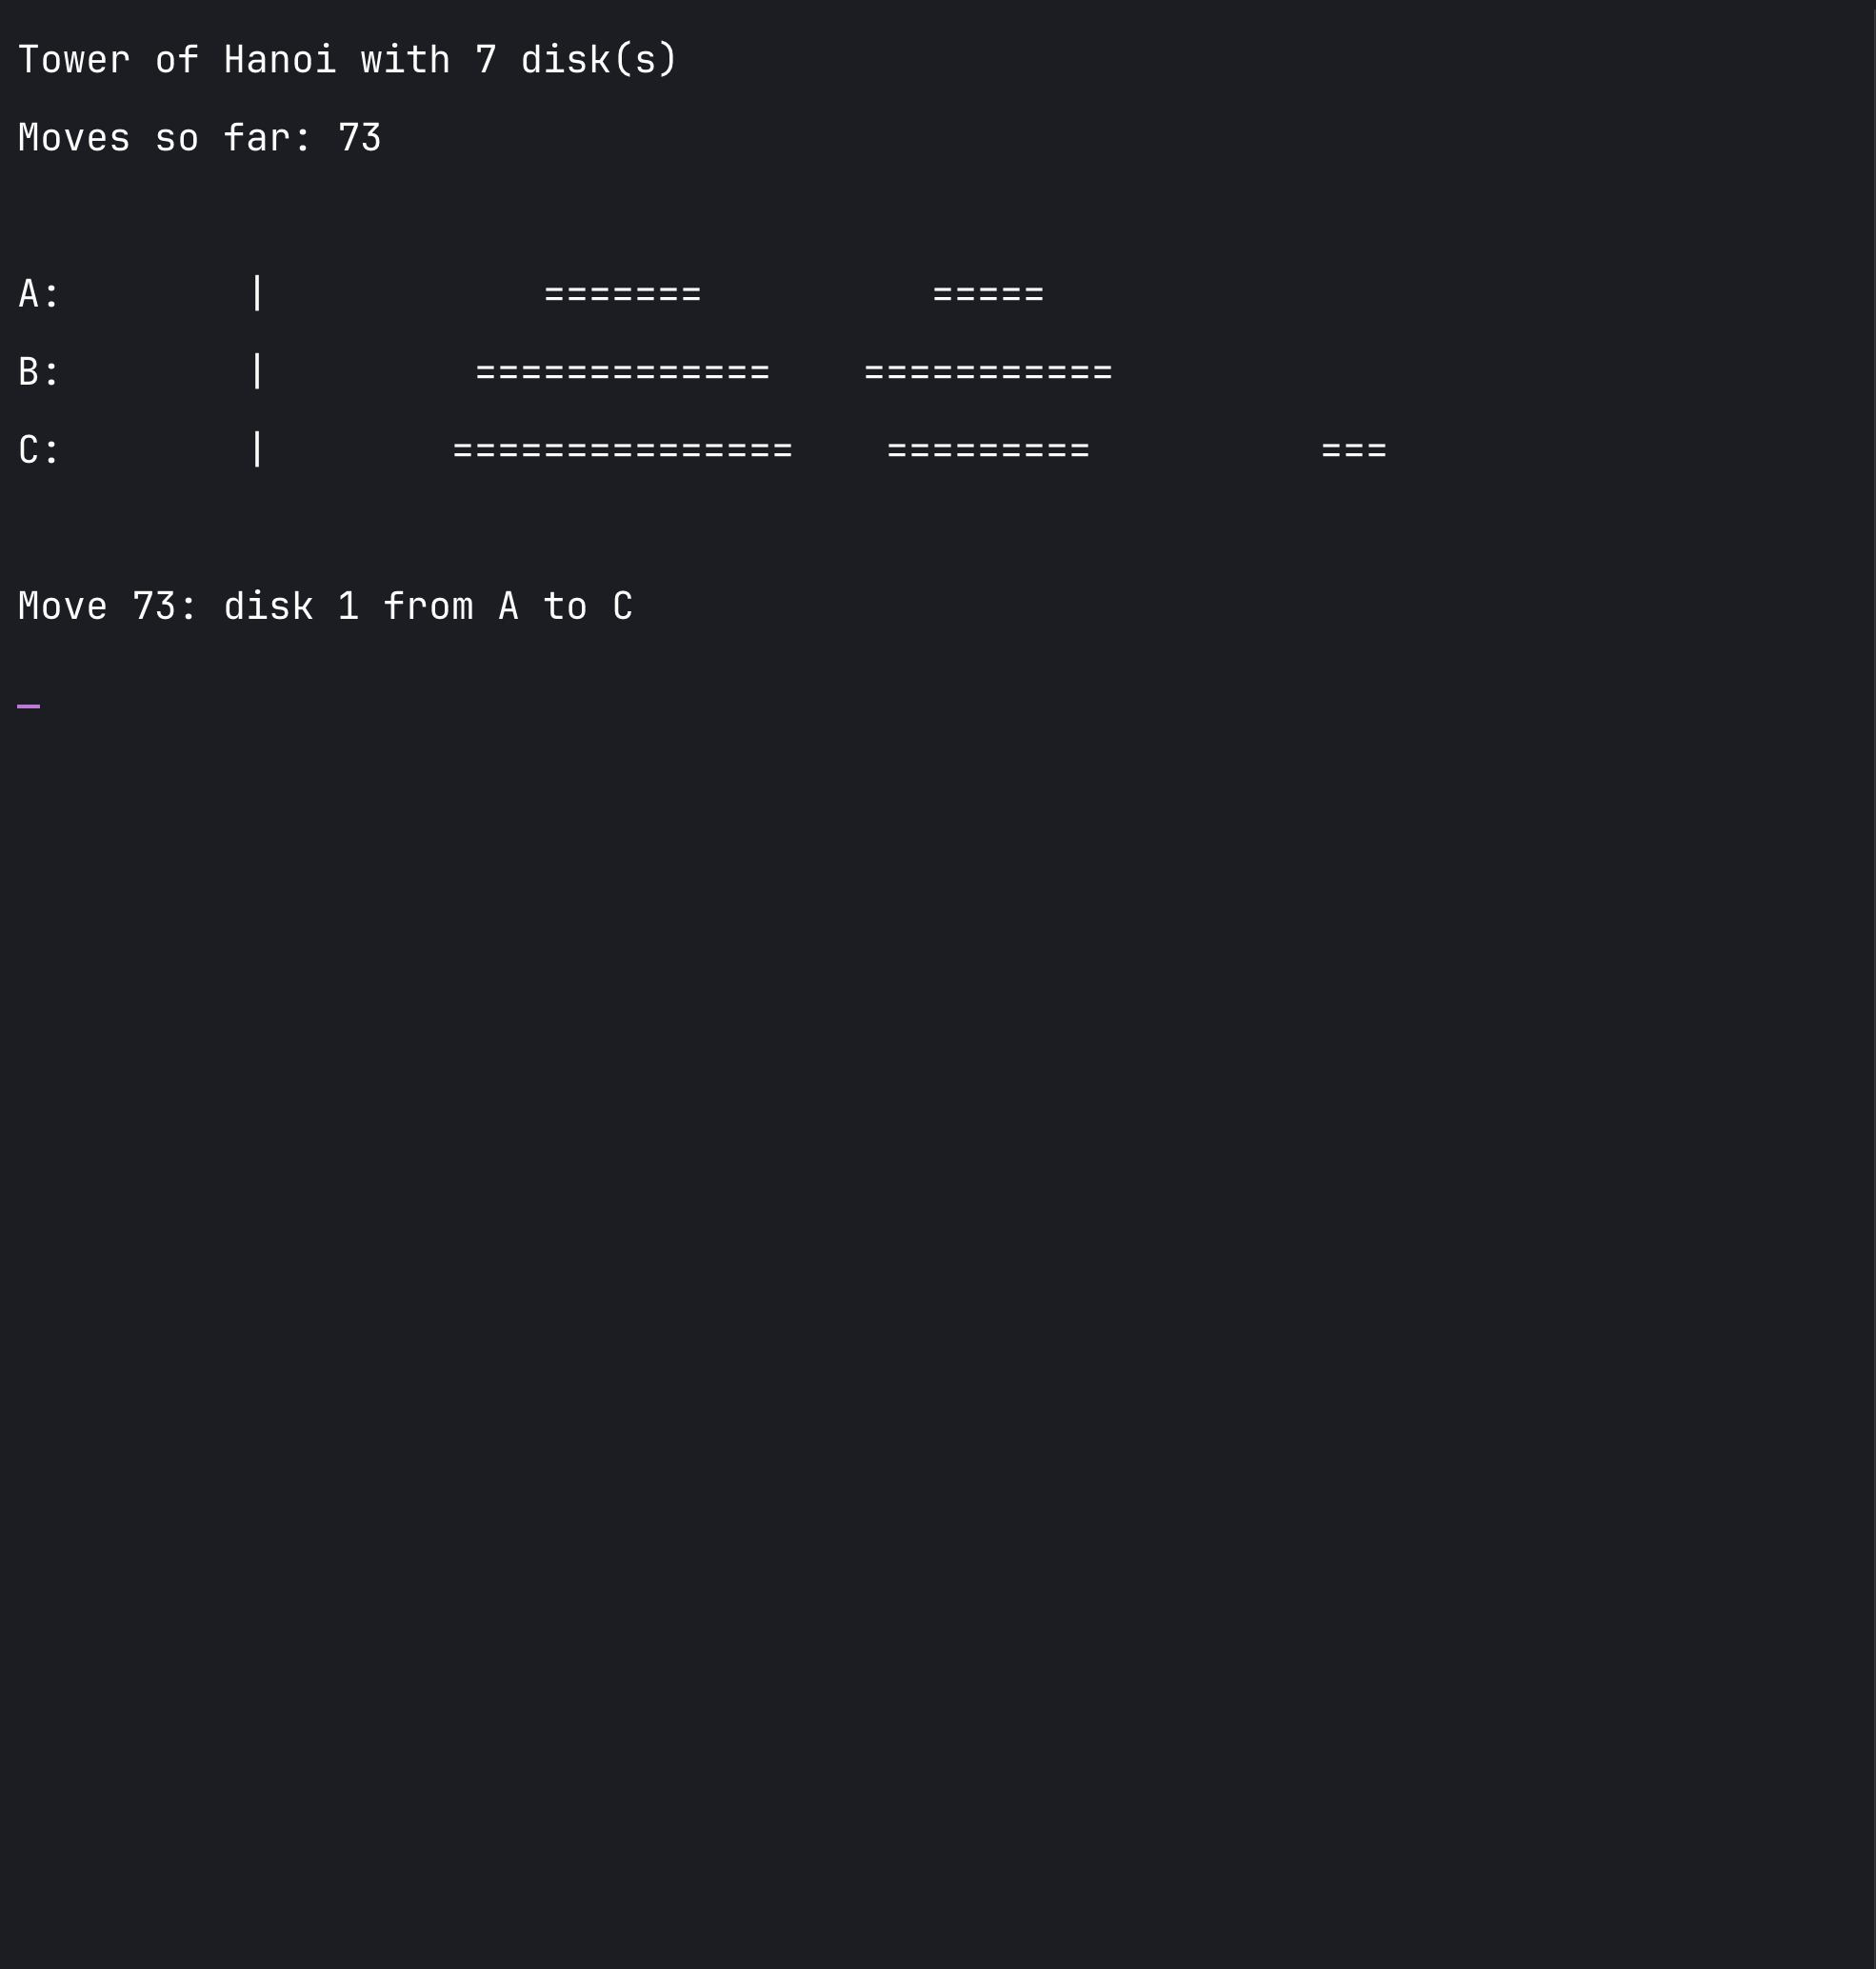
\includegraphics[width=0.78\textwidth]{hanoi.png}
  \caption{Tower of Hanoi terminal demonstration in Bash}
\end{figure}

\section{Conway's Game of Life Demo}

The Conway's Game of Life implementation is contained in \texttt{life.sh}. It simulates cell evolution across multiple generations on a small grid rendered directly in the terminal. Live cells are drawn as \texttt{[]} and dead cells are drawn as blank space.

\subsection{Concept Demonstrated}

The key algorithmic concept demonstrated here is \textbf{iteration}. The script repeatedly traverses the grid to:

\begin{itemize}[leftmargin=1.5em]
  \item count the live neighbors of each cell,
  \item apply Conway's birth and survival rules,
  \item render the next generation.
\end{itemize}

The iterative sections are called out in the code comments inside:

\begin{itemize}[leftmargin=1.5em]
  \item \texttt{count\_neighbors()}
  \item \texttt{render\_board()}
  \item \texttt{step\_generation()}
\end{itemize}

\subsection{Example Output}

\begin{figure}[h]
  \centering
  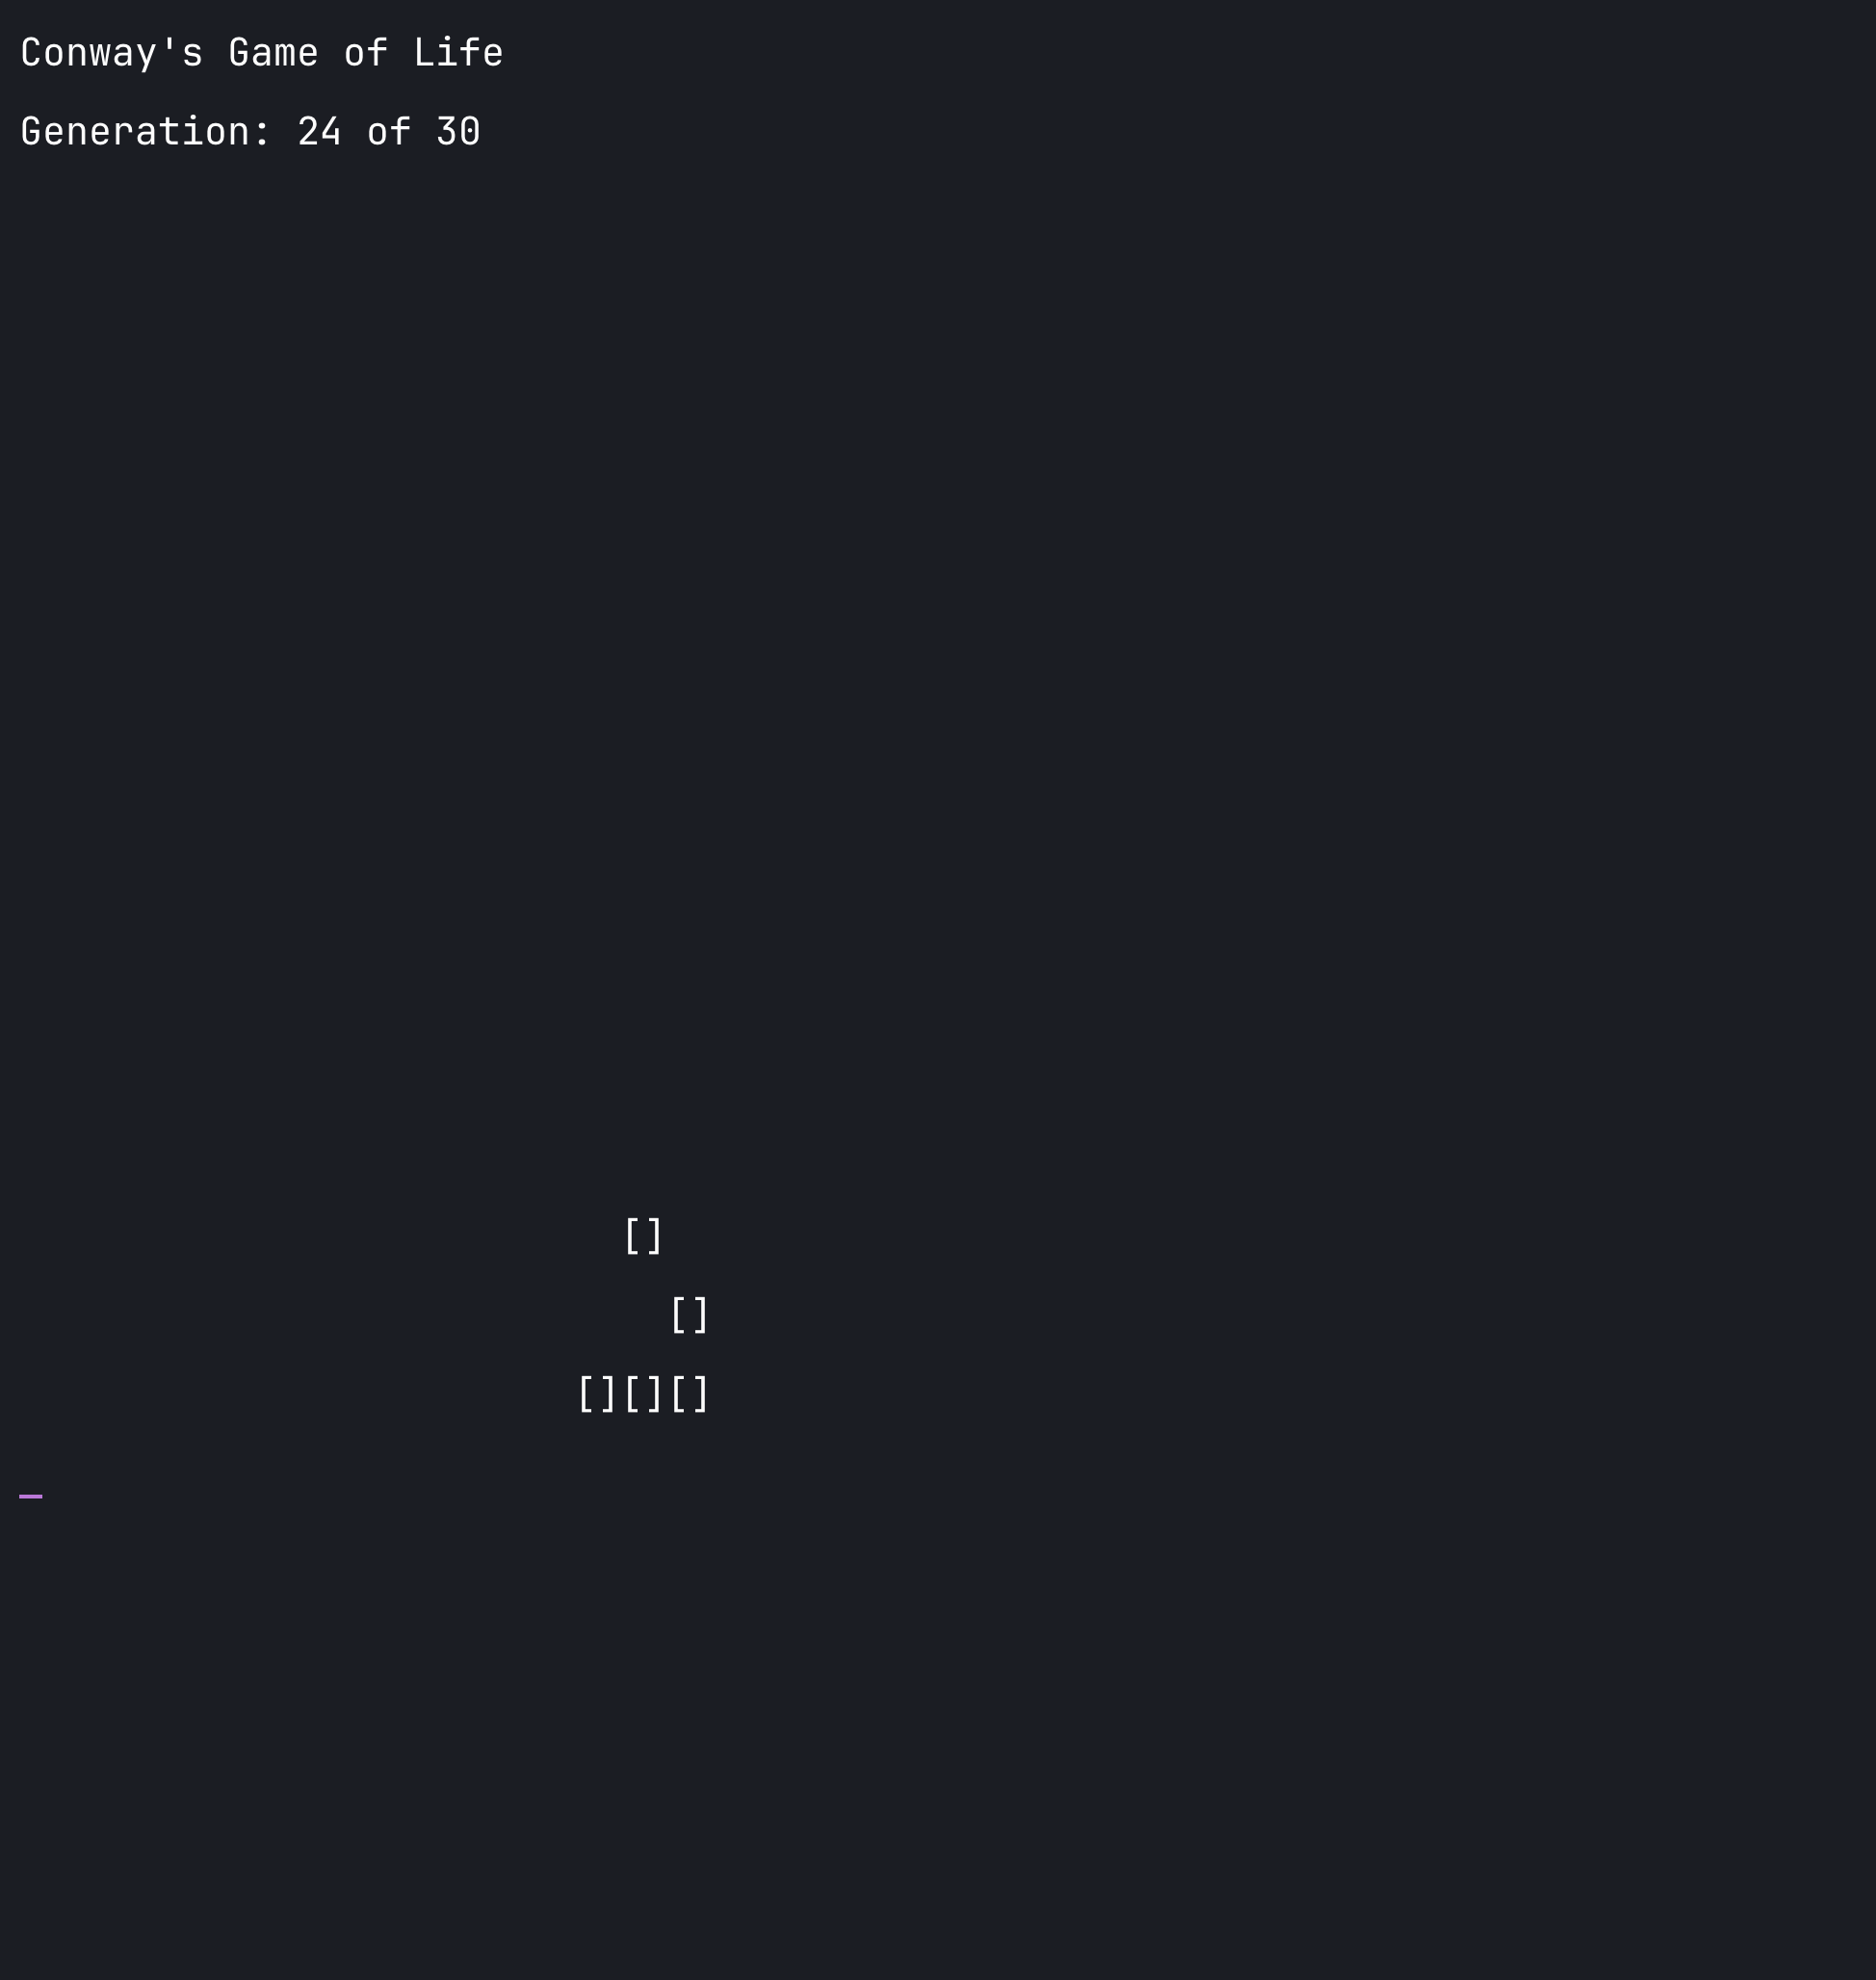
\includegraphics[width=0.78\textwidth]{game_of_life.png}
  \caption{Conway's Game of Life terminal demonstration in Bash}
\end{figure}

\section{Public Website}

The assignment noted that publishing the work publicly was optional. To support that, this repository also includes a small static website built with:

\begin{itemize}[leftmargin=1.5em]
  \item \texttt{index.html}
  \item \texttt{style.css}
  \item \texttt{script.js}
\end{itemize}

This website is designed for GitHub Pages and provides browser-based visualizations of both demos. The Bash scripts remain the primary assignment deliverables, while the website serves as a public-facing showcase.

\begin{figure}[h]
  \centering
  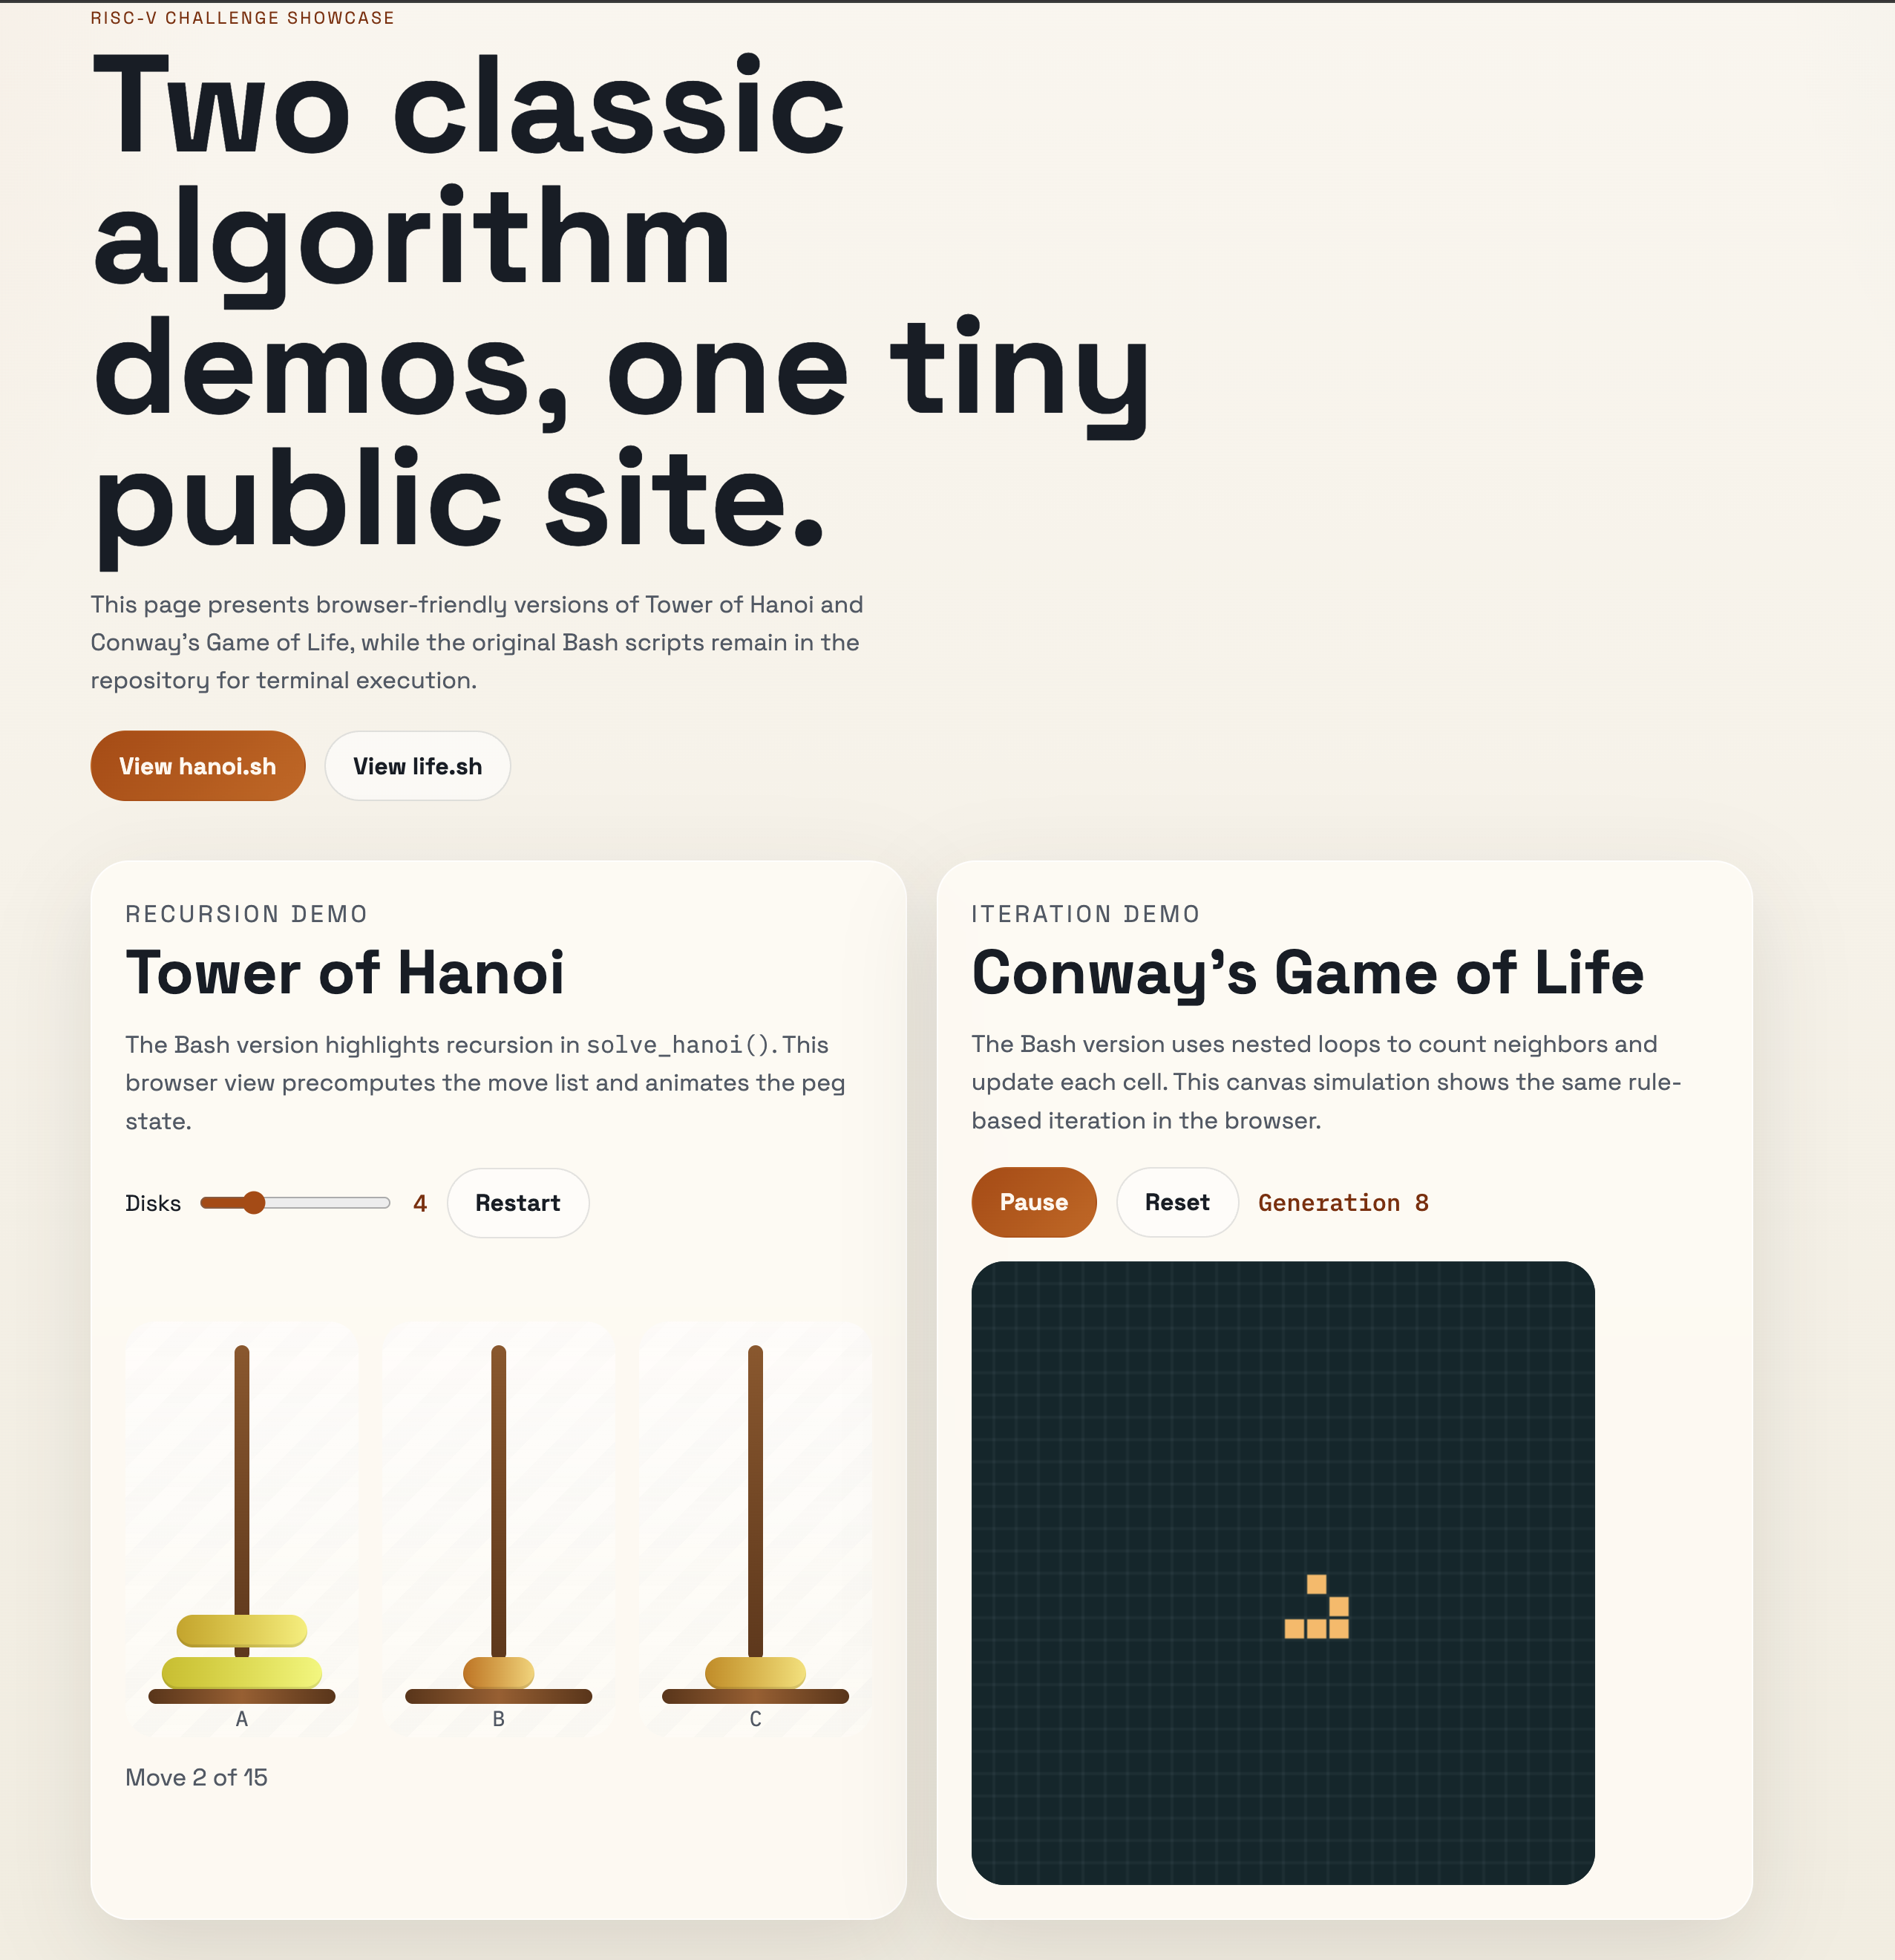
\includegraphics[width=0.82\textwidth]{website.png}
  \caption{GitHub Pages website showcasing both demos}
\end{figure}

\clearpage

\section{Files Included}

\begin{lstlisting}
hanoi.sh
life.sh
index.html
style.css
script.js
.github/workflows/pages.yml
README.md
report.tex
hanoi.png
game_of_life.png
website.png
\end{lstlisting}

\clearpage
\appendix

\section{Complete Source Code}

This appendix includes the full code used for the challenge submission so that the PDF is self-contained.

\subsection{\texttt{hanoi.sh}}

\lstinputlisting[caption={Tower of Hanoi Bash implementation}]{hanoi.sh}

\clearpage
\subsection{\texttt{life.sh}}

\lstinputlisting[caption={Conway's Game of Life Bash implementation}]{life.sh}

\clearpage
\subsection{\texttt{index.html}}

\lstinputlisting[caption={GitHub Pages HTML entrypoint}]{index.html}

\clearpage
\subsection{\texttt{style.css}}

\lstinputlisting[caption={GitHub Pages stylesheet}]{style.css}

\clearpage
\subsection{\texttt{script.js}}

\lstinputlisting[caption={Browser demo logic for both visualizations}]{script.js}

\clearpage
\subsection{\texttt{.github/workflows/pages.yml}}

\lstinputlisting[caption={GitHub Actions workflow for Pages deployment}]{.github/workflows/pages.yml}

\end{document}
